\chapter{Exploraci\'on de los datos, control de calidad y preprocesado}



\section{Exploraci\'on visual de los datos}
Los gr\'aficos son \'utiles para comprobar la calidad de los datos de microarrays,
obtener informaci\'on sobre c\'omo se deben preprocesar los datos y comprobar, finalmente, que el preprocesado se haya realizado correctamente.

Se debe tener en cuenta que aunque la base del proceso es similar, los procedimientos espec\'ificos var\'ian considerablemente dependiendo de
si tratamos con datos obtenidos a partir de arrays de un o dos colores (Affymetrix o ADNc).

\begin{itemize}
 \item Arrays de dos colores (ADNc)

Tradicionalmente los arrays de dos colores o de ADNc se realizan de forma menos automatizada que los de un color o de Affymetrix.
Esto implica que, tras obtener la imagen, el escaneado del archivo ``.TIFF''
\footnote{.TIFF es un formato para archivos de imagen de alta calidad} resultante puede ser llevado a cabo mediante un \emph{software} independiente
como \texttt{Genepix}.
Este programa convierte las im\'agenes en n\'umeros y genera un archivo de informaci\'on (con extensi\'on ``.gpr'') a partir del cual pueden
calcularse las expresiones relativas, as\'i como valores de calidad para cada \emph{spot} o punto escaneado en la imagen.

Para cada imagen (o sea para cada microarray) hay un archivo .gpr que contiene una fila por gen y
varias columnas con distintos valores, por ejemplo la intensidad para cada canal, valores resumen de las intensidades y
controles de calidad (``FLAGS'').

Los valores de intensidad se convierten en una \'unica \emph{matriz de expresi\'on} que contiene una columna por chip
con los valores de intensidad relativa $(\log\left (R/G \right ))$ y una fila por gen (mismas filas que archivos .gpr).


\item Arrays de un color (Affymetrix)

EL procesado de archivos de Affymetrix se realiza de forma autom\'atica por su sistema de an\'alisis. El resultado de escanear la imagen es un
archivo ``.CEL'' que, a diferencia de los arrays de dos colores est\'a en formato binario es decir que solo puede ser le\'ido con programas
espec\'ificos para ello.

De forma similar a los arrays de dos colores, se genera un archivo .CEL por chip, que contiene los valores PM (\emph{perfect match}) y
MM (\emph{mismatch}) para cada sonda y marcadores de presencia/ausencia (una por grupo de sondas).

A partir de las intensidades de los archivos .CEL se genera la matriz de expresi\'on que contiene una columna por chip
con los valores de intensidad absoluta y una fila por grupo de sondas.


\end{itemize}

\subsection{Gr\'aficos de diagn\'ostico para chips de ADNc}

El diagn\'ostico de arrays de dos canales se basa principalmente
en la imagen y en diferentes tipos de gr\'aficos.

\begin{itemize}
 \item Imagen del array

Esta imagen nos ofrece una visi\'on r\'apida de la calidad del array, d\'andonos informaci\'on
acerca del balance del color, la uniformidad en la hibridaci\'on y en los \emph{spots},
de si el background es mayor del normal y dela existencia de artefactos como el polvo o peque\~nas marcas (rasgu\~nos).

\item Scatterplots

La normalizaci\'on es un punto clave en el proceso de an\'alisis de microarrays y
se ha dedicado un gran esfuerzo a desarrollar y probar diferentes m\'etodos
(\cite{Quackenbush:2003,Yang:2002a}). Una raz\'on para ello es que hay
diferentes artefactos t\'ecnicos que deben ser corregidos para poder ser
utilizados, y no cualquier m\'etodo puede funcionar con todos ellos.

En general, los m\'etodos de normalizaci\'on se basan en el siguiente principio: La
mayor parte de los genes en un array se pueden expresar o no expresar ante
cualquier condici\'on, pero se espera que s\'olo  una peque\~na cantidad de genes muestre cambios de
expresi\'on entre condiciones.

Esto da una idea de como deber\'ia ser un gr\'afico de intensidades. Por ejemplo, si
no hubiese artefactos t\'ecnicos, en arrays de dos canales, una gr\'afica de
dispersi\'on de intensidad del rojo frente al verde deber\'ia dejar la mayor parte
de los puntos alrededor de una diagonal. Cualquier desviaci\'on de esta situaci\'on
deber\'ia ser atribuible a razones t\'ecnicas, no biol\'ogicas, y por tanto, deber\'ia
ser eliminada. Esto ha conducido a un m\'etodo de normalizaci\'on muy popular
consistente en estimar la transformaci\'on a aplicar, como una funci\'on de las
intensidades utilizando el m\'etodo \emph{lowess} en la representaci\'on transformada de la
gr\'afica de dispersi\'on conocida como \emph{gr\'afica MAplot}.

Figure \ref{fig:C05normScatterMA} (a) muestra una gr\'afica de dispersi\'on del canal
rojo frente al verde en un array. El hecho de que los
datos no est\'en centrados alrededor de la diagonal sugiere la necesidad de
normalizaci\'on. Una representaci\'on muy popular que ayuda a visualizar mejor esta
asimetr\'ia es la gr\'afica MAplot
(\ref{fig:normScatterMA}(b)). Geom\'etricamente representa una rotaci\'on de la
gr\'afica de dispersi\'on, en la que el significado de los nuevos ejes es:

\begin{itemize}
\item $A=\displaystyle \frac{1}{2}(\log_2 (R*G))$: El logaritmo de la intensidad media de los dos
canales,

\item $M=\log_2 \displaystyle \frac{R}{G}$: El logaritmo de la expresi\'on relativa entre
ambos canales (normalmente conocido como ''log--ratio'').
\end{itemize}


\vspace{-0.5cm}
\begin{figure}[!h]
\titolfigura[0cm]{Figura \ref{fig:c05normScatterMA}. (a) Gr\'afico de  R vs G  (b) MAplot (intensidad vs
  log-ratio)}
\label{fig:c05normScatterMA}
\fbox{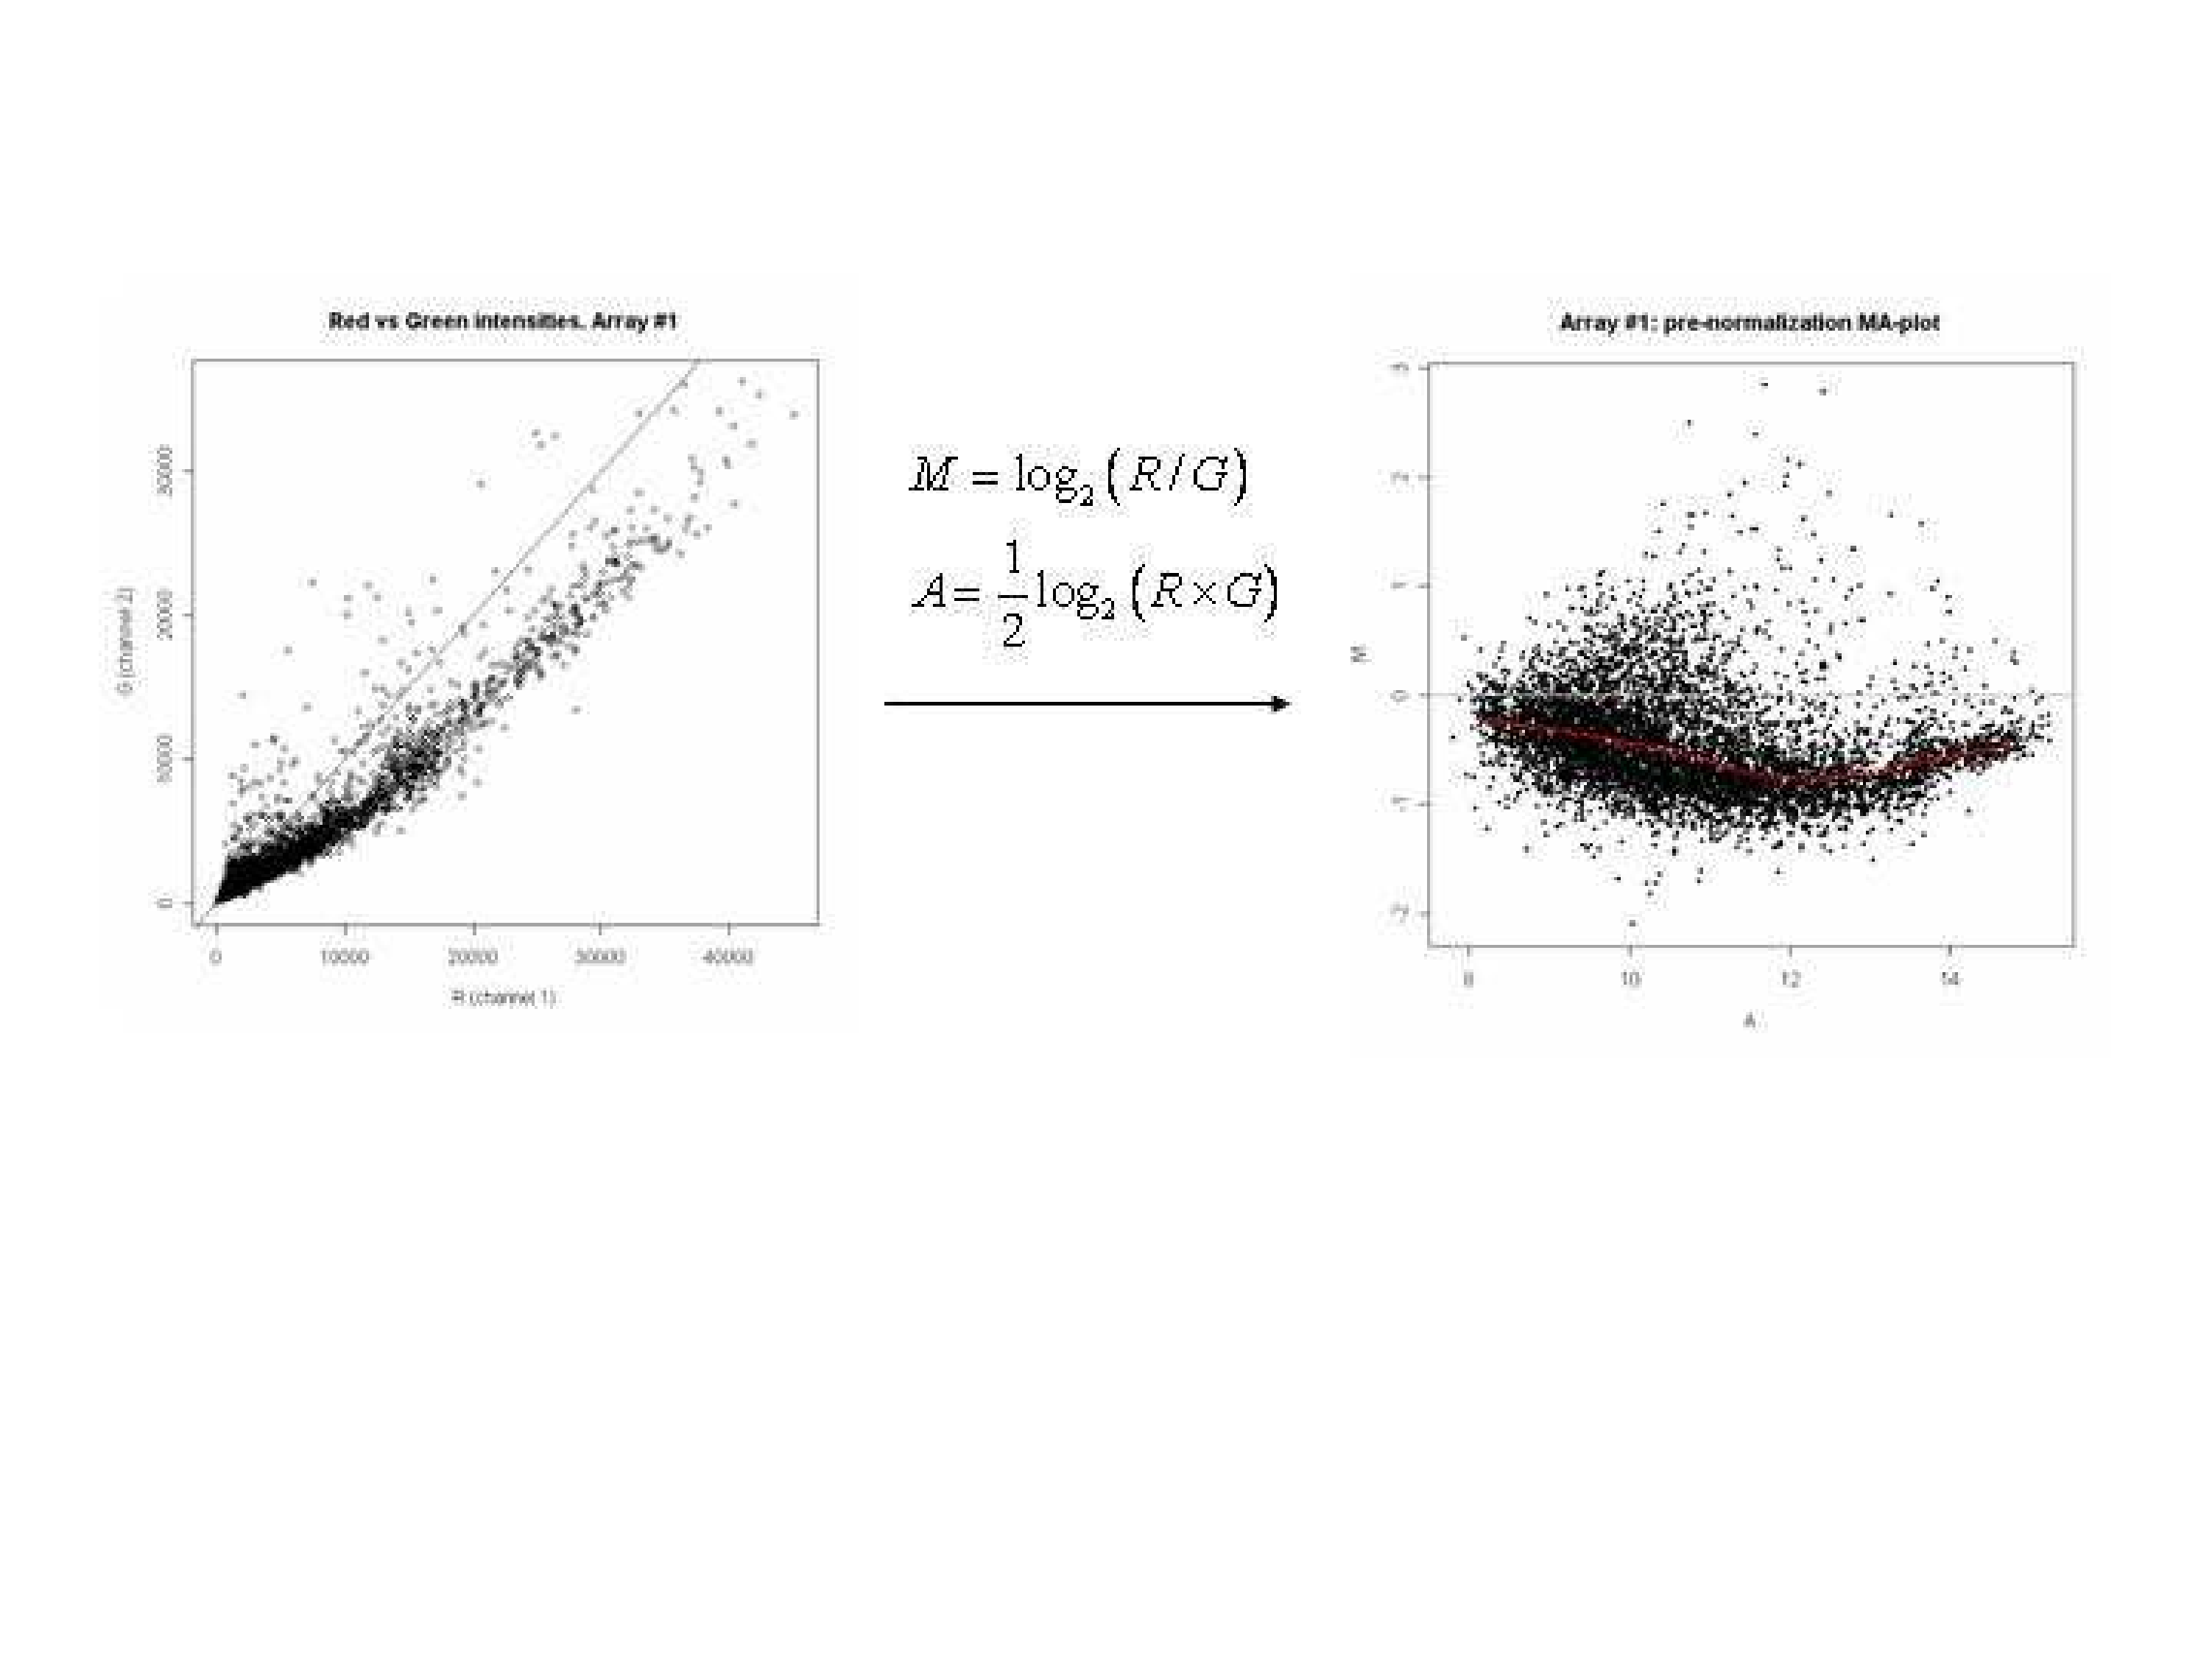
\includegraphics[height=6cm,width=0.98\linewidth]{epsimages/c05normScatterMA.eps}}
\end{figure}

 \item Histogramas de se\~nales y de la relaci\'on se\~nal/ruido

\'Utiles para detectar posibles anormalidades o un background excesivamente alto (Figure \ref{c05signalNoise}).


\textD{Figura \ref{c05signalNoise}}{\'Util para detectar posibles anormalidades o un background excesivamente alto}

\vspace{-0.5cm}
\begin{figure}[!h]
\titolfigura[0cm]{Figura \ref{c05signalNoise}. Im\'agenes de buena calidad, como se puede ver en el gr\'afico superior,
deber\'ian tener un background bajo y una alta relaci\'on se\~nal/ruido. Im\'agenes de
mala calidad, gr\'afico inferior, muestran un background alto y baja relaci\'on
se\~nal/ruido.}
\label{c05signalNoise}
\fbox{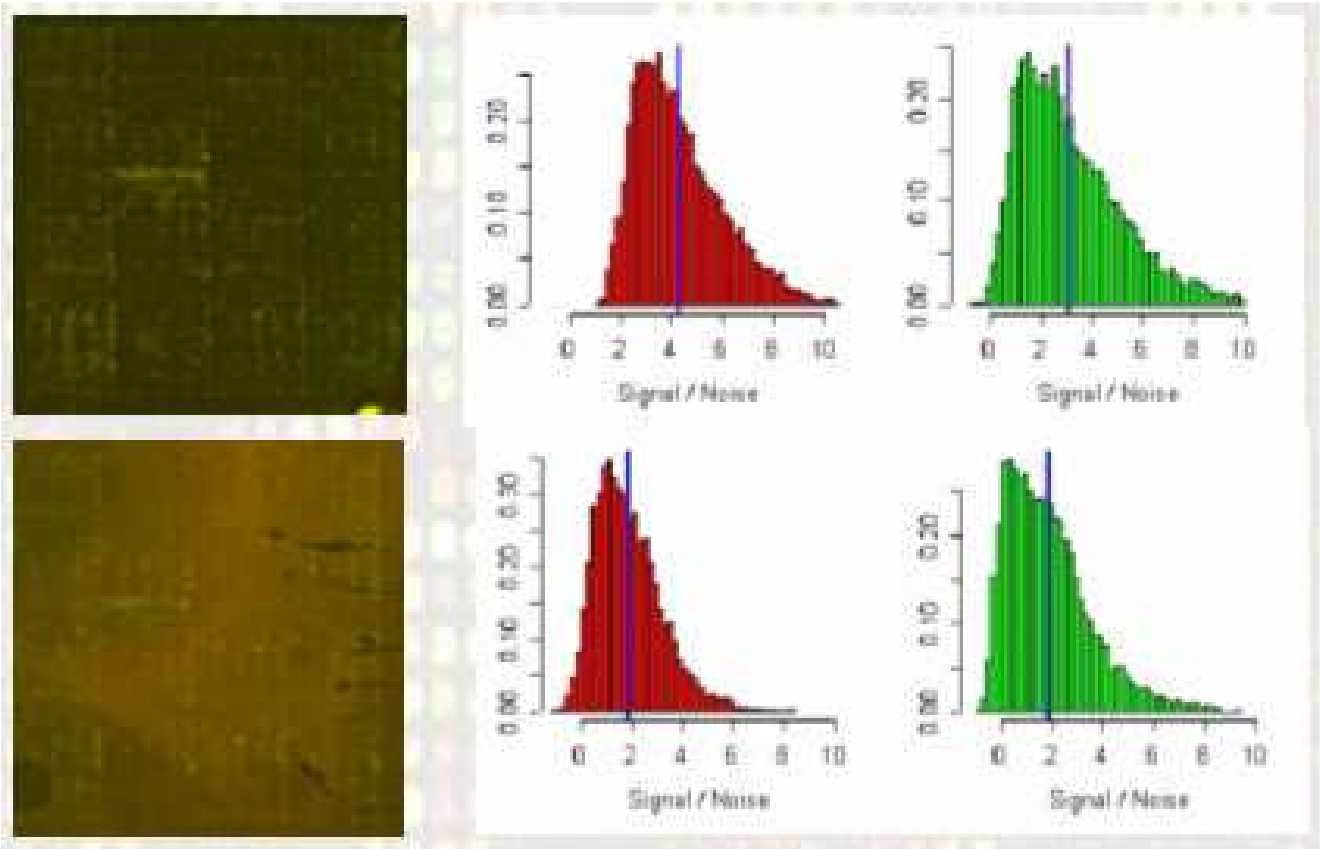
\includegraphics[height=6cm,width=0.98\linewidth]{epsimages/c05signalNoise.eps}}
\end{figure}

 \item Boxplots

Un gr\'afico muy utilizado es el boxplot m\'ultiple con una caja por cada chip. Del
alineamiento (o falta de \'el) y la semejanza (o disparidad) entre las cajas, se deduce si hace
falta, o no, normalizar entre arrays.

%incluir imagen
\end{itemize}



\subsection{Gr\'aficos de diagn\'ostico para chips de Affymetrix}

La imagen del array de Affymetrix s\'olo es \'util para evidenciar grandes problemas como burbujas, ara\~nazos, etc.
Puede hacerse a partir de intensidades o de residuos a ajustar modelos PLM (ver m\'as adelante).


\textD{Figura \ref{c05plotAffy}}{La imagen del array de Affymetrix s\'olo es \'util para evidenciar grandes problemas como burbujas, ara\~nazos, etc}

\vspace{-0.5cm}
\begin{figure}[!h]
\titolfigura[0cm]{Figura \ref{c05plotAffy}. Im\'agenes donde se pueden observar ara\~nazos, burbujas, etc.}
\label{c05plotAffy}
\fbox{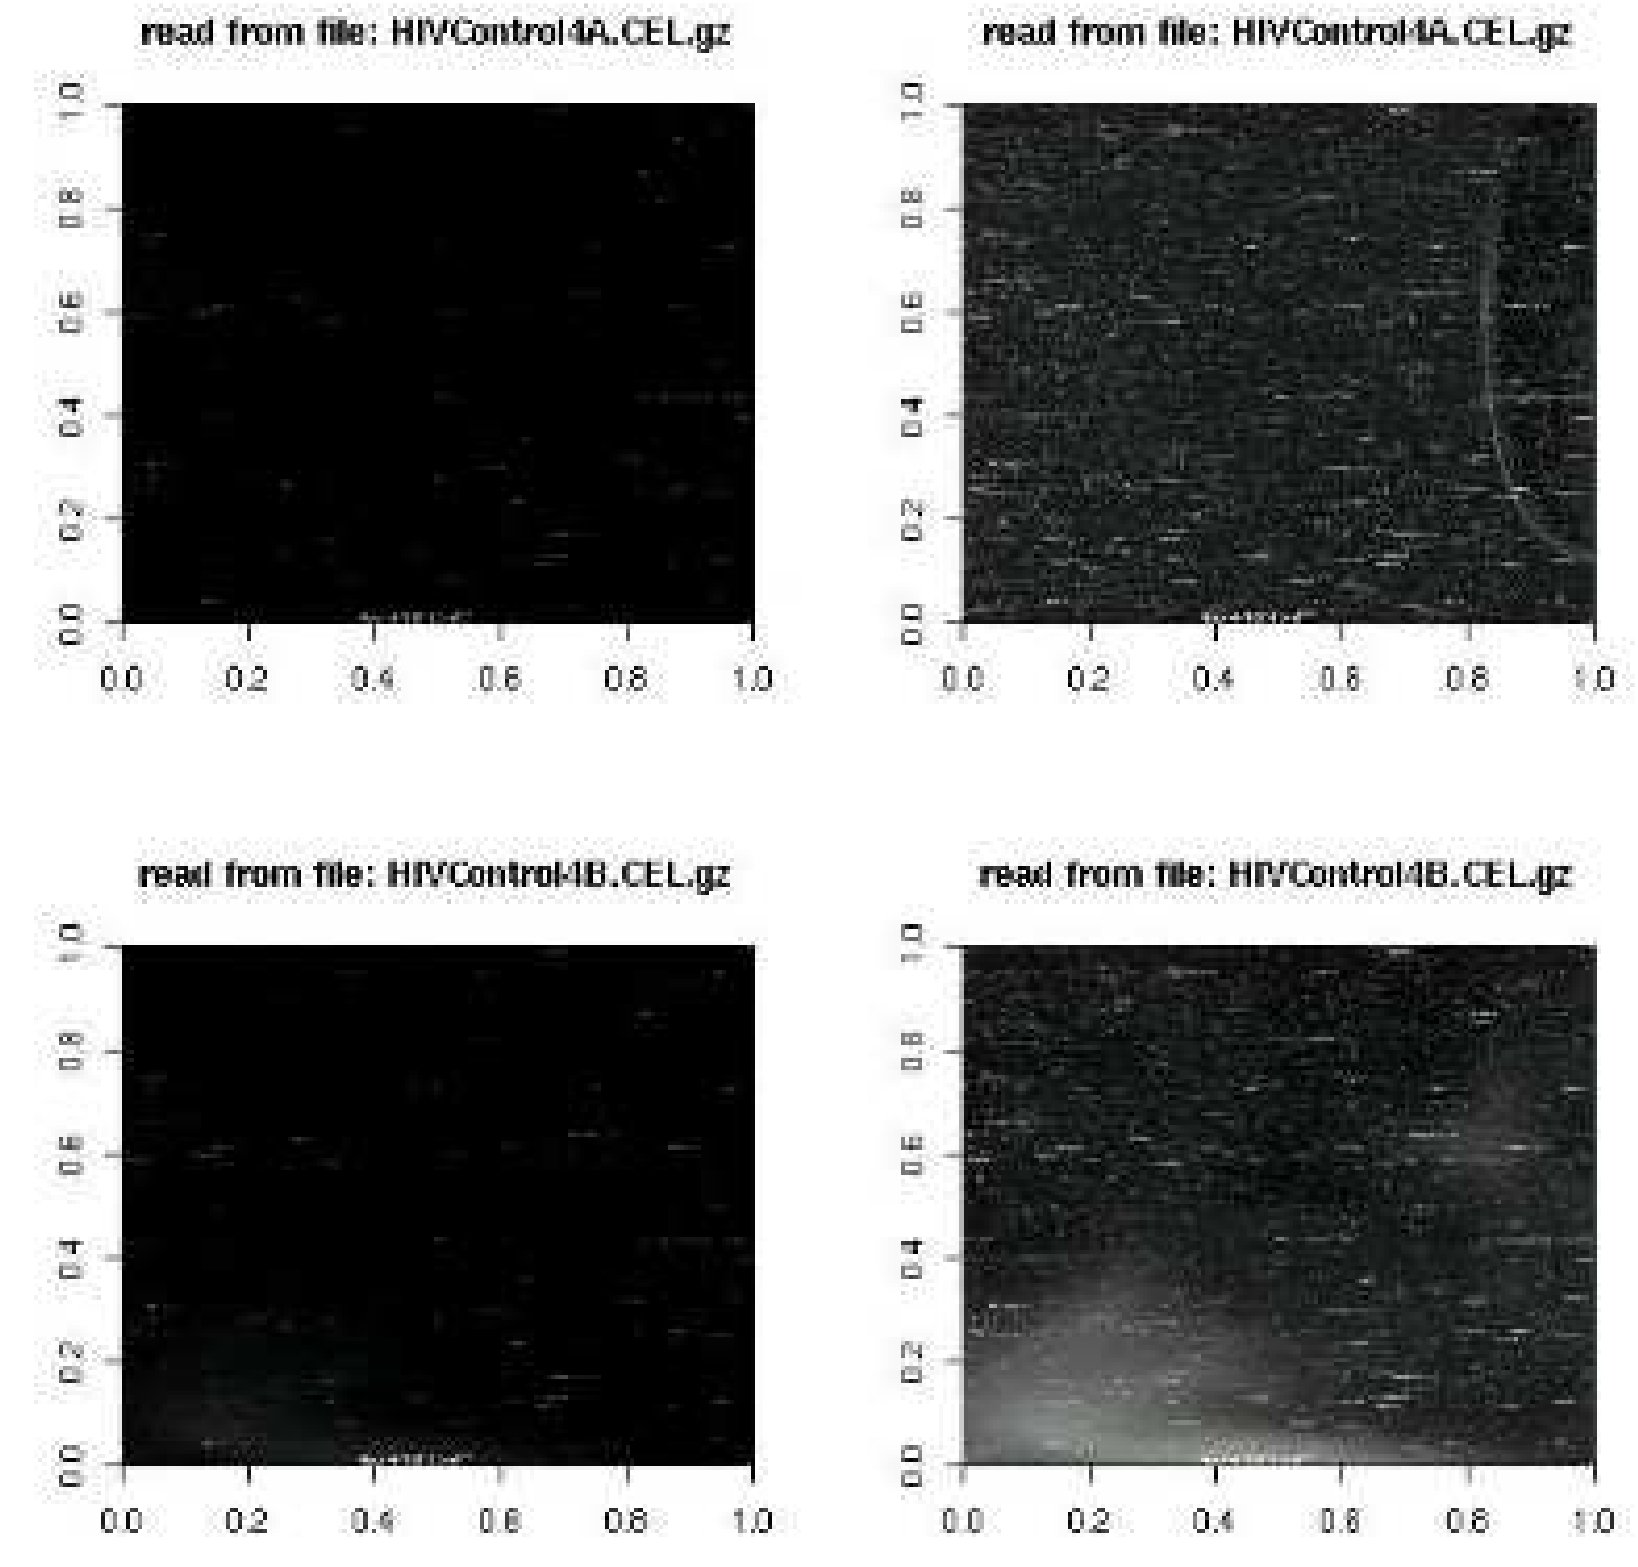
\includegraphics[height=6cm,width=0.98\linewidth]{epsimages/c05plotAffy.eps}}
\end{figure}

Los gr\'aficos utilizados para el diagn\'ostico en este tipo de arrays son:
\begin{itemize}
 \item MAplot de un canal

En los chips de ADNc el MAplot se utliza para comparar los dos canales en cada array (rojo y verde). En cambio, en
los chips de Affymetrics, en que s\'olo hay un canal en cada array,  la \'unica forma de definir M (el log ratio) es a partir de la comparaci\'on  entre pares de de valores, uno de ellos corresponde al array de estudio y el otro es un valor de referencia que suele ser la media de todos los arrays.(Figure \ref{c05MAPlotAffy}).


\textD{Figura \ref{c05MAPlotAffy}}{En los chips de Affymetrix la \'unica forma de definir M (el log ratio) es comparar entre
diferentes arrays}

\vspace{-0.5cm}
\begin{figure}[!h]
\titolfigura[0cm]{Figura \ref{c05MAPlotAffy}. MAplot de un canal}
\label{c05MAPlotAffy}
\fbox{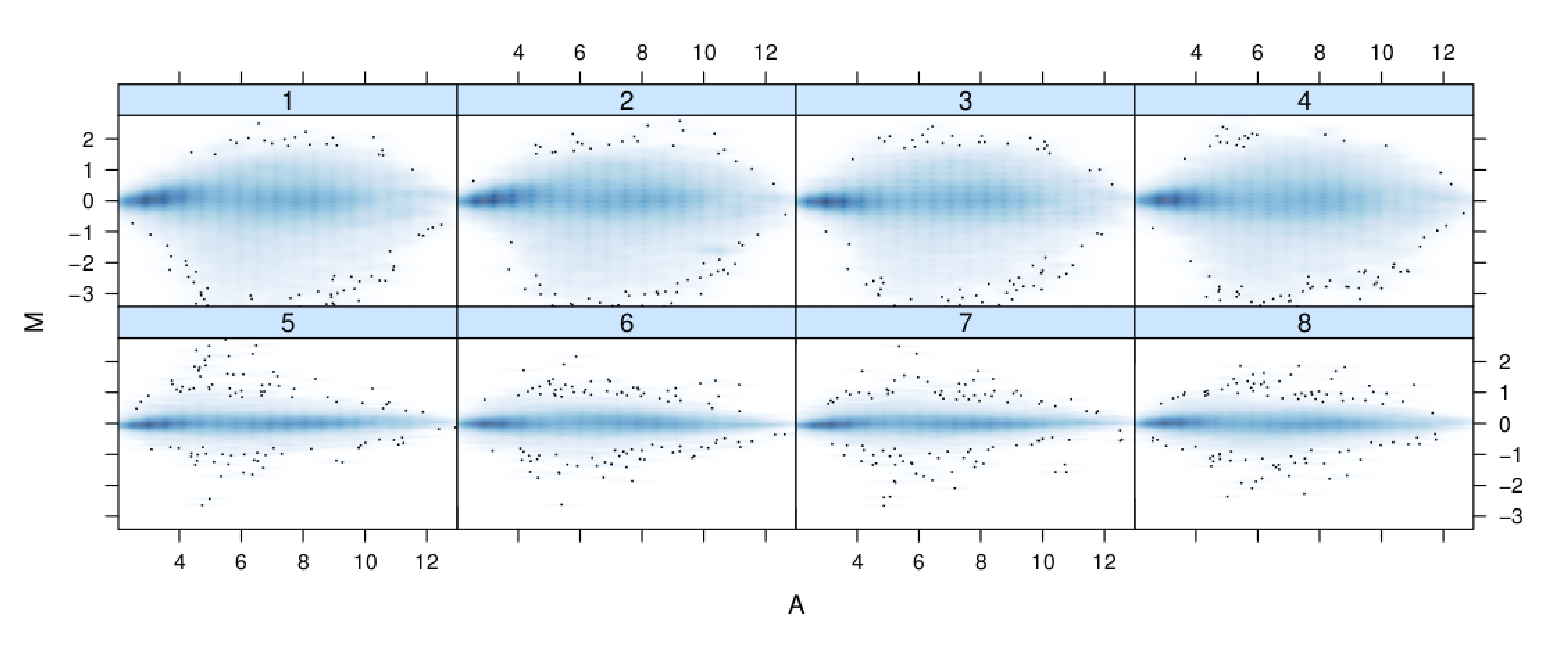
\includegraphics[height=6cm,width=0.98\linewidth]{epsimages/c05MAPlotAffy.eps}}
\end{figure}

$M=\log_2(I_1) - \log_2(I_2)$: log ratio
$A=\displaystyle \frac{1}{2}(\log_2 (I_1)+\log_2(I_2))$: log de intensidades
Donde $I_1$ es la intensidad del array de estudio, e $I_2$ es la intensidad media de arrays.
Por lo general, se espera que la distribuci\'on en el gr\'afico se concentre a lo largo del eje M = 0.


 \item Boxplots

Representan las distribuciones de intensidad de los arrays.
Cada caja corresponde a un array. Por lo general, se espera que las cajas sean similares. Si la distribuci\'on de un array es muy diferente de
los dem\'as, esto puede indicar un problema en el experimento.

\textD{Figura \ref{c05BoxPlotAffy}}{Los Boxplots representan las distribuciones de intensidad de los arrays}

\vspace{-0.5cm}
\begin{figure}[!h]
\titolfigura[0cm]{Figura \ref{c05BoxPlotAffy}. Boxplots}
\label{c05BoxPlotAffy}
\fbox{\includegraphics[height=6cm,width=0.98\linewidth]{epsimages/c05BoxPlotAffy.eps}}
\end{figure}

 \item Gr\'aficos de densidad

Muestran la estimaci\'on de la densidad (a partir del  histograma) de los datos.
Por lo general, las distribuciones de los arrays deber\'ian tener formas y rangos similares. Los arrays cuyas distribuciones son muy
diferentes al resto deben ser considerados como arrays con posibles problemas.


 \item Gr\'aficos de degradaci\'on

Indican la calidad de la hibridaci\'on del ARN a lo largo de los conjuntos de sondas.

\textD{Figura \ref{c05DenDigPlot}}{ Gr\'aficos de diagn\'ostico de densidad y de degradaci\'on}

\vspace{-0.5cm}
\begin{figure}[!h]
\titolfigura[0cm]{Figura \ref{c05DenDigPlot}.}
\label{c05DenDigPlot}
\fbox{\includegraphics[height=6cm,width=0.98\linewidth]{epsimages/c05DenDigPlot.eps}}
\end{figure}


    \item Modelos de bajo nivel (``Probe-Level-Models'' o PLM)


Los modelos de bajo nivel (``Probe-Level-Models'' o PLM) ajustan a los valores de intensidad --a nivel de sondas, no de valores totalizados de gen-- un modelo explicativo. Los valores estimados por este modelo se comparan con los valores reales y se obtienen los errores o ``residuos'' del ajuste. El an\'alisis de dichos residuos procede de forma similar a lo que se realiza al analizar un modelo de regresi\'on:
Si los errores no presentan ning\'un patr\'on especial supondremos que el modelo se ajusta relativamente bien.
Si, en cambio, observamos desviaciones de esta presunta aleatoriedad querr\'a decir que el modelo no explica bien las observaciones, lo cual se atribuir\'a a la existencia de alg\'un problema con los datos.

Con los valores ajustados del modelo se calculan dos medidas:

\begin{itemize}
\item La expresi\'on relativa en escala logar\'itmica `` Relative Log Expression'' (RLE) es una medida estandarizada de la expresi\'on.
No es de gran utilidad pero deber\'ia presentar una distribuci\'on similar en todos los arrays.
\item El error no estandarizado y normalizado o ``NUSE'' es el m\'as informativo ya que representa la distribuci\'an de los residuos a la que
hac\'iamos referencia m\'as arriba.
Si un array es problem\'atico la caja correspondiente en el boxplot aparece desplazada hacia arriba o abajo de las dem\'as.
\end{itemize}

\end{itemize}


\section{Normalizaci\'on de arrays de dos colores}
La palabra \emph{normalizaci\'on} describe las t\'ecnicas utilizadas para transformar adecuadamente los datos antes de que sean analizados.
El objetivo es corregir diferencias sistem\'aticas entre muestras, en la misma o entre im\'agenes, lo que no representa
una verdadera variaci\'on entre las muestras biol\'ogicas.

Estas  diferencias sistem\'aticas pueden deberse, entre otras, a:
\begin{itemize}
 \item Cambios en la tinci\'on que producen sesgos  la intensidad del \emph{spot}.
\item La ubicaci\'on en el array que puede afectar el proceso de lectura. 
\item Un problem en la placa de origen.
\item La existencia de diferencias en la calidad de la impresi\'on: pueden presentarse  variaciones en  los pins y el tiempo de impresi\'on
\item Camio en los par\'ametros de la digitalizaci\'on (escaneo).
\end{itemize}

A veces puede ser dif\'icil detectar estos problemas , aunque existen algunas  formas de saber  si es necesaria realizar una normalizaci\'on. Aqui destacamos dos posibilidades:
\begin{enumerate}
\item Realizar una auto-hibridaci\'on.
Si hibridamos una muestra con ella misma, las intensidades deber\'ian ser las mismas en ambos canales.
Cualquier desviaci\'on de esta igualdad, significa que hay un sesgo sistem\'atico.

\item Detectar artefactos espaciales en la imagen o en la tinci\'on de los gr\'aficos
de diagn\'ostico

\end{enumerate}
\subsection{M\'etodos de normalizaci\'on}


\subsubsection{\textbf{Normalizaci\'on global}}

Este m\'etodo esta basado en un ajuste global, es decir en modificar todos los valores una cantidad \emph{c}, estimada de acuerdo a alg\'un criterio.
\begin{equation}
 \log_2 R/G \rightarrow \log_2 R/G-c=\log_2 R/(Gk)
\end{equation}
opciones para $k$ o $c= \log_2k$ son

$c$= mediana o media de log ratio para un conjunto concreto de genes o genes control o genes housekeeping.

La intensidad total de la normalizaci\'on

$k=\sum R_i/\sum G_i$
%imagen ejemplo de Callow

\subsubsection{\textbf{Normalizaci\'on dependiente de la intensidad}}
En este caso se realiza una modificaci\'on espec\'ifica para cada valor. Esta modificaci\'on se obtiene como una funci\'on de la intensidad total del gen ($c=c(A)$).
\begin{equation}
 \log_2 R/G \rightarrow \log_2 R/G-c(A)=\log_2 R/(Gk(A))
\end{equation}

Una posible estimaci\'on de esta funci\'on puede hacerse utilizando la funci\'on \emph{lowess} (LOcally WEighted  Scatterplot Smoothing).

\section{``Sumarizaci\'on'' y normalizaci\'on microarrays de Affymetrix}


En los arrays de Affymetrix, como en todos los tipos de microarrays, tras escanear la imagen se obtiene una serie de valores de
intensidad de cada elemento del chip.
En el caso de estos arrays sabemos que cada valor no corresponde a la expresi\'on de un gen:

\begin{itemize}
\item Hay m\'ultiples valores (sondas o ''probes``) por cada gen, que originan un \emph{probeset}.
\item Cada grupo de sondas  consiste en m\'ultiples pares de sondas, donde cada puede tener  dos elementos:
\subitem Un ''perfect match`` que coincide exactamente con el fragmento del gen al que corresponde la sonda
\subitem Un ''mismatch`` que que coincide con el anterior salvo por el valor central que se ha sustitu\'ido por el nucle\'otido complementario.
Estos ``mismatches' se introdujeron en los primeros arrays de affymetrix para tener una medida de hibridaci\'on no espec\'ifica pero en las versiones m\'as recientes se han abandonado.

\end{itemize}


El proceso que convierte las se\~nales individuales en valores de expresi\'on normalizados para cada gen consta de tres etapas:
\begin{enumerate}
\item Correcci\'on del ruido de fondo o ''background``
\item Normalizaci\'on para hacer los valores comparables
\item ''Sumarizaci\'on``(Resumen) o concentraci\'on de los valores de cada grupo de sondas en un \'unico valor de expresi\'on absoluto normalizado
para cada gen.
\end{enumerate}
A menudo los tres pasos se denominan gen\'erica -y err\'oneamente- ''normalizaci\'on``.

A diferencia de los chips de ADNc, aqu\'i las medidas de expresi\'on son absolutas (no se compara una condici\'on contra otra)
dado que cada chip se hibrida con un \'unica muestra.

Hay muchos m\'etodos para estimar la expresi\'on (m\'as de 30 publicados).
Cada m\'etodo contempla de forma expl\'icita o impl\'icita las tres formas de preprocesado: correcci\'on del fondo,
normalizaci\'on y resumen.

Los principales m\'etodos que consideraremos son:
\begin{itemize}
\item Microarray Suite (MAS). M\'etodo oficial de Affymetrix. Versiones 4.0 y 5.0
\item dChip: Li and Wong. M\'etodo basado en modelos multichip.
\item RMA (Bioconductor). Actualmente es el m\'etodo ''est\'andar``.
\end{itemize}

\subsection{M.A.S. 4.0}

Es el primer m\'etodo introducida por Affymetrix.
La correcci\'on del fondo se realiza restando el ''perfect match`` del ''mismatch``
\begin{equation}
 E_j=PM_j-MM_j
\end{equation}
La normalizaci\'on se realiza de forma global haciendo transformaciones de forma que la media de todo el chip sea la misma y
la sumarizaci\'on se basa en calcular el promedio de las diferencias absolutas ignorando los pares que se desv\'ian m\'as de $3\sigma$ de $\mu$.
\begin{equation}
 Dif. Media=\frac{1}{|A|}\sum_{j \in A}(PM_j-MM_j)
\end{equation}
Los problemas que presenta estem\'etodo son:
\begin{itemize}
\item 1/3 de los MM son mayores que los PM
\item Pueden aparecer valores MM negativos
\item El uso de los MM a\~nade ruido
\end{itemize}

\subsection{M.A.S. 5.0}

Todo esto ha llevado a sustituirlo por otra variante, el MAS 5.0, llamado as\'i por venir implementado en el
software de affymetrix llamado ''MicroArray Suite 5.0``.

Este m\'etodo utiliza un estad\'istico robusto, \emph{el biweight de Tukey}, para corregir y ponderar el fondo y
calcular (estimar) la se\~nal.
El biweight de Tukey $T_{bi}$ pondera los valores por su distancia a la mediana, es decir,
mide la tendencia central pero realiza un ajuste de outliers.

La l\'ogica de este m\'etodo reside en pensar que el valor de MM no siempre tiene sentido, (p.ej si MM $>$ PM).
Dado que esto sucede en ocasiones se realiza el cambio siguiente:
\begin{enumerate}
\item Se introduce el background espec\'ifico de un conjunto de pruebas $i$ de tama\~no $n$ basado en los pares de pruebas $j$:
\begin{equation}
 SB_i=T_{bi}(\log(PM_{i,j})-\log(MM_{i,j})): j= 1,\ldots,n
\end{equation}
\item SB se utiliza para decidir como se ajusta el background
\begin{itemize}
\item Si es grande los datos suelen ser fiables
\item Si es peque\~no mejor basarse tan solo en PM
\end{itemize}
\end{enumerate}
Este m\'etodo no tan solo corrige el background sino que tambi\'en permite normalizar y sumarizar.
Para ello se introduce el ''Mismatch Idealizado`` (IM) que permite corregir la intensidad de las pruebas individuales. 
Este m\'etodo tambi\'en ha sido muy criticado:
\begin{itemize}
\item Se considera que no tiene mucho sentido promediar las pruebas entre arrays, pues \'estos pueden tener caracter\'isticas
de hibridaci\'on intr\'insecamente distintas.
\item El m\'etodo no mejora ''aprendiendo`` del funcionamiento entre arrays de las pruebas individuales.
\end{itemize}

\subsection{Modelos multichip de Li y Wong}

De aqu\'i surgi\'o la idea de ajustar modelos basados en multiples arrays o modelos ''multi-chip``.
Los primeros en introducirlo fueron Cheng Li \& Wing Wong (2001) introduciendo el resumen de la intensidad de las pruebas basado en modelos.

Los valores de expresi\'on dentro de un conjunto de sondas son muy estables entre arrays, es decir,
es menor la variabilidad inter-chips que intra-chips. Su m\'etodo se basa en la Modelizaci\'on de las pruebas a nivel de se\~nal individual, suponiendo que la se\~nal de cada prueba es proporcional a:
\begin{itemize}
\item Cantidad de muestra diana (\emph{target}):  $\theta_i$
\item Afinidad de la secuencia espec\'ifica de la prueba por la diana: $\phi_j$

Gran afinidad no significa gran especificidad, una sonda puede dar una se\~nal alta con una diana y
tambi\'en con otras secuencias (muy afin y poco espec\'ifica)
\end{itemize}

Asumiendo las suposiciones anteriores y tomando como base de la estimaci\'on la diferencia $PM_{ij}-MM_{ij}$
se obtiene el modelo multiplicativo:
\begin{equation}
PM_{ij}-MM_{ij}=\phi_j \theta_i + \varepsilon_{ij}
\end{equation}

La estimaci\'on se realiza utilizando m\'etodos robustos con eliminaci\'on de outliers y
re-estimaciones sucesivas hasta la convergencia.

Una de las cr\'iticas al modelo de Li-Wong es que el modelo supone homocedasticidad, es decir, que la distribuci\'on
de los errores tiene varianza constante, y en la pr\'actica, la mayor\'ia de medidas biol\'ogicas, presentan errores dependientes de la intensidad, a mayor valor suelen tener mayor varianza.


\subsection{El m\'etodo RMA (Robust Multi-Array Average)}

Para compensar algunas deficiencias del m\'etodo de dChip, Irizarry et al. introducen un m\'etodo basado
en la modelizaci\'on lineal del logaritmo del modelo anterior con la estimaci\'on basada en m\'etodos de estad\'istica robustos.

Este m\'etodo se ha convertido en el est\'andar ''de facto`` actualmente por  muchos usuarios de Bioconductor.

Esquem\'aticamente los pasos que realiza este m\'etodo son:
\begin{enumerate}
\item Ajusta el fondo (background) bas\'andose solo en los valores PM y utilizando un modelo estad\'istico complejo
en el que combina la modelizaci\'on de la se\~nal y del background.
\item Toma logaritmos base 2 de cada intensidad ajustada por el background.
\item Realiza una normalizaci\'on por cuantiles de los valores del paso 2 entre todos los chips.
\item Estima las intensidades de cada gen separadamente para cada conjunto de sondas. Para ello realiza una t\'ecnica similar
a una regresi\'on robusta denominada ''median pulish'' sobre una matriz de datos que tiene los arrays en filas y los grupos
de sondas en columnas.
\end{enumerate}

Como resultado final de todos los pasos anteriores se obtiene la matriz con los  datos sumarizados y normalizados.


\section{Filtraje no espec\'ifico}


El filtraje no espec\'ifico es recomendable para eliminar el ruido de fondo y limitar los ajustes posteriores a los necesarios.
Los principales procesos de filtrado son:
\begin{itemize}
 \item Eliminanci\'on de los spots marcados como err\'oneos mediante  flags y que son debidos  a problemas en la hibridaci\'on o en el escaneo.
 \item Eliminanci\'on de spots con se\~nales muy bajas debido a problemas en el \emph{spotting} o a que no ha habido hibridaci\'on en ese spot (Filtraje pr ).
\item Eliminaci\'on de genes que no presenten una variaci\'on significativa en su se\~nal, entre distintas condiciones experimentales (Filtraje por variabilidad).
Ante la duda,\emph{se debe ser conservador y reducir la operaci\'on de filtraje al m\'inimo}
\end{itemize}
El objetivo del filtraje es eliminar aquellos spots cuyas im\'agenes o se\~nales sean err\'oneas por diferentes motivos, disminuyendo el ruido
de fondo. Aunque existe controversia a su uso, prefiriendo el no filtrado a eliminar de forma no intencionado spots informativos.







